% !TEX root = ../main.tex

\section{Validation of the FW-H Method for Monopole Sources} \label{sec:monopole_validation}
The first investigation are of monopole with stationary, as well as co-translating source and observer. This gives a baseline sensitivity of different control surface grid resolutions and time step sizing. The radius of the control surface is set to $1m$, and the observer is located at $[50,50,0]$. In the the co-translation case, the points are translating at $150m/s$ along the x-direction.

For grid sensitivity, the control surface is discretised with $40 \times 40$, $15 \times 15$, and $5\times5$ grids and the time step size is set to $dt=0.005s$. Conversely, for the time step sizing test, the grids are set to $40\times40$ resolution while the time steps are sized to $dt=0.005s$, $dt=0.025s$, and $dt=0.125s$, which correspond to $200 Hz$, $40 H$z, and $8 Hz$ sampling frequencies, respectively.

\begin{figure}[H]
    \centering
    \begin{subfigure}[b]{0.495\textwidth}
        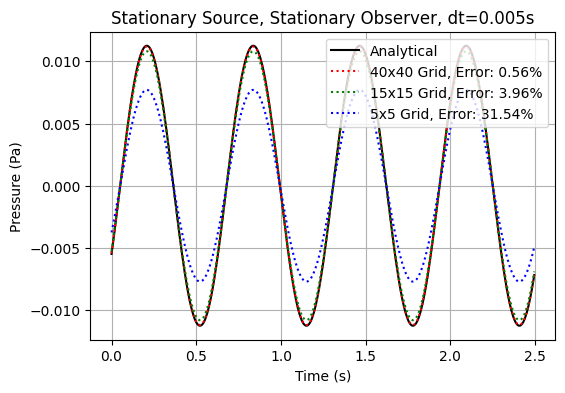
\includegraphics[width=\textwidth]{fig_monopole/monopole_stationary_dx.png}
        \caption{}
        \label{fig:monopole_ss_dx}
    \end{subfigure}
    \hfill
    \begin{subfigure}[b]{0.495\textwidth}
        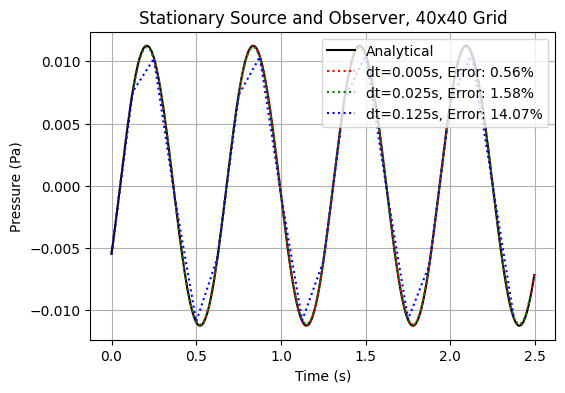
\includegraphics[width=\textwidth]{fig_monopole/monopole_stationary_dt.png}
        \caption{}
        \label{fig:monopole_ss_dt}
    \end{subfigure}

    \vspace{0.25cm}

    \begin{subfigure}[b]{0.495\textwidth}
        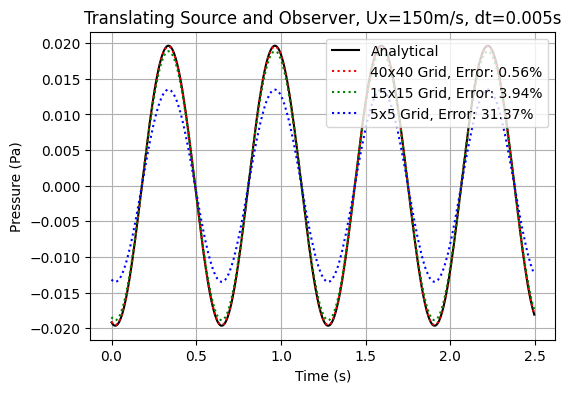
\includegraphics[width=\textwidth]{fig_monopole/monopole_moving_so_dx.png}
        \caption{}
        \label{fig:monopole_tt_dx}
    \end{subfigure}
    \hfill
        \begin{subfigure}[b]{0.495\textwidth}
        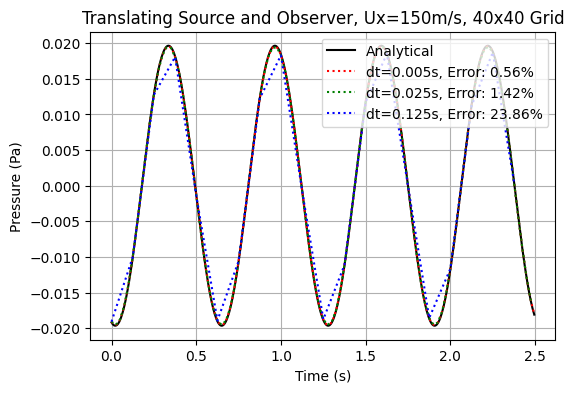
\includegraphics[width=\textwidth]{fig_monopole/monopole_moving_so_dt.png}
        \caption{}
        \label{fig:monopole_tt_dt}
    \end{subfigure}

    \caption[Stationary and zero co-translating monopole test cases]{\centering Stationary and co-translating monopole test cases, a) stationary with varied grid sizing, and b) stationary with varied time-stepping sizing, c) co-translating with varied grid sizing, and d) co-translating  with varied time-stepping sizing}
    \label{fig:monopole_zero_relative}
\end{figure}

For the relative motion case, the grid and time-stepping sensitivity set ups remain the same. The cases differ by translating only the source at $150m/s$ along the x-axis, while the observer remains stationary.

\begin{figure}[H]
    \begin{subfigure}[b]{0.495\textwidth}
        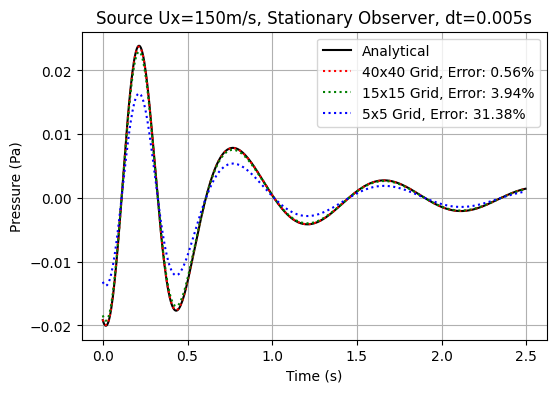
\includegraphics[width=\textwidth]{fig_monopole/monopole_moving_s_dx.png}
        \caption{}
        \label{fig:monopole_ts_dx}
    \end{subfigure}
    \hfill
    \begin{subfigure}[b]{0.495\textwidth}
        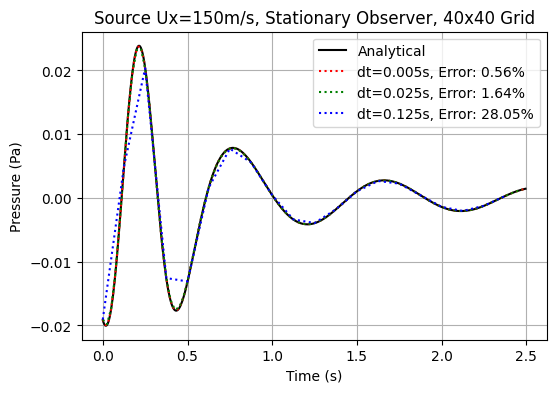
\includegraphics[width=\textwidth]{fig_monopole/monopole_moving_s_dt.png}
        \caption{}
        \label{fig:monopole_ts_dt}
    \end{subfigure}
    \caption[Translating monopole with stationary observer test case]{\centering Translating monopole with stationary observer test case, a) with varied grid sizing, and b) with varied time-step sizing}
    \label{fig:monopole_relative}
\end{figure}

Comparing the first two cases (Figure \ref{fig:monopole_zero_relative}) shows a distinction in amplitude and phase, despite both scenarios having zero relative Mach number ($M_r=0$). In the co-translating case, the source moves through the quiescent fluid medium, which causes a phase shift of $\sim\pi/2$ and pressure increase due to the convective term. Furthermore, the emission distance $r$ in the retarded time, $\tau = t - r/c$, differs from the geometric distance because both points are moving through the medium during the propagation time. The third case demonstrates the effect of relative Mach number. In Figure \ref{fig:monopole_relative} the Doppler effect causes the acoustic frequency and pressure amplitude received by the observer to increase as the source approaches ($0\leq t\leq 0.33s$), and decrease as it moves away ($t>0.33s$).

In the grid resolution comparisons, while the finest resolution of $40\times40$ has very good agreement with the analytical solutions at less than $1\%$ error in all cases, the errors progressively increase to $\sim4\%$ and $\sim 30\%$, for coarser resolutions. The plots show at lower resolution, the numerical results could not capture the peaks and troughs of the harmonic wave, causing dissipation. Given the acoustic wavelength is $\sim214m$ (from the prescribed frequency and speed of sound values), the coarsest grid has an arc distance between two nodes of 1.25 meters. The errors shown in the grid sensitivities are mainly due to geometric error of the spherical domain, rather than the grids not being able to capture the wavelengths. This shows that this grid resolution is sufficient given the input and control surface radius.

The time step sensitivity study exhibits similar trends. The $dt=0.005s$ and $dt=0.025s$ sizes yield errors at less than $1\%$ and $2\%$, respectively. However, largest time-step size of $dt=0.125s$ (an $8Hz$ sampling frequency), is insufficient to capture the input acoustic frequency of $10rad/s$ or $\sim1.6Hz$, as it can only sample at five times the input. This can be seen in the lags in the plots as the numerical solution attempted to keep up with the wave.